\documentclass[department=ds, notes={hide notes}, slidesperpage=1]{beamerruhuisstijl}

% Force pretty font
\usepackage[utf8]{inputenc}
\usepackage[english]{babel}
\usepackage{lmodern}
\usepackage[T1]{fontenc}
\usepackage[babel=true]{microtype}

\title{Roerei}
\subtitle{
	Premise selection for Coq\\
	\\
	Wouter Geraedts
}

\date{\today}

\usepackage{listings}
\usepackage{color}
\usepackage{xspace}

\usepackage{tikz}

\usepackage{pgfplots}
\usepackage{pgfplotstable}

\begin{document}
\renewcommand{\dept}{icis}
\begin{frame}
	\titlepage
\end{frame}

\begin{frame}{Outline}
	\begin{itemize}
		\item What is Automated Theorem Proving?
		\item Machine Learning for Automated Theorem Proving
		\item Competing with the State of the Art
	\end{itemize}
\end{frame}

% \begin{frame}{Logic}
% 	\begin{minipage}{0.5\textwidth}
% 		\begin{itemize}
% 			\item All men are mortal.
% 			\item Socrates is a man.
% 			\item Therefore, Socrates is mortal.
% 		\end{itemize}
% 	\end{minipage}
% 	\hspace{2em}
% 	\begin{minipage}{0.4\textwidth}
% 		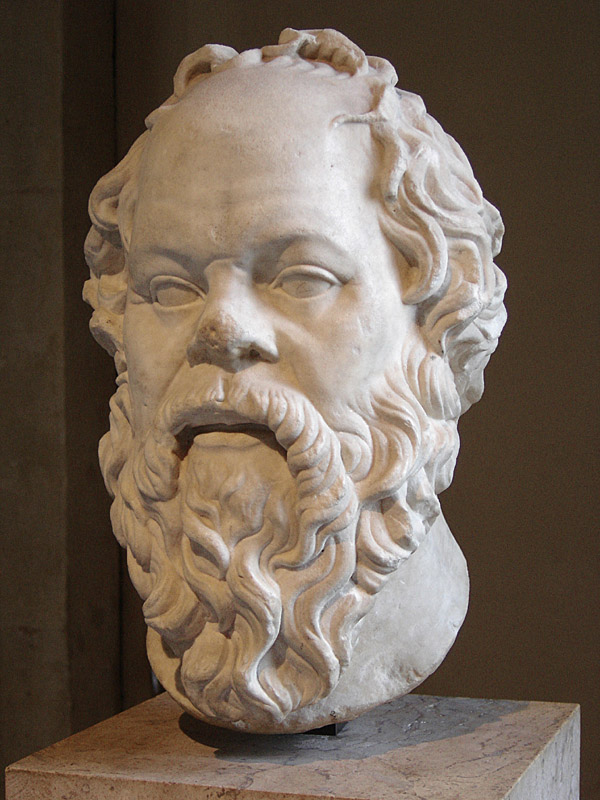
\includegraphics[width=1.0\textwidth]{figures/socrates.jpg}\\
% 		\centering \color{gray}{Eric Gaba (CC by-nc-sa 2.5)}
% 	\end{minipage}
% \end{frame}

% \begin{frame}{CASC}
% \begin{block}{Higher order (THF)}
% \begin{tabular}{p{3.6cm}|rrr}
% 	\textbf{Prover}    & \textbf{Solved} & \textbf{Time}  \\ \hline
% 	\textbf{Satallax MaLeS 1.3} & \textbf{333/400}         & \textbf{18.88} \\
% 	Satallax 2.7       & 324/400         & 5.68 \\
% 	Isabelle 2013      & 316/400         & 38.91 \\
% 	LEO-II             & 269/400         & 7.21 \\
% 	agsyHOL 1.0        & 236/400         & 5.83 \\
% 	HOLyHammer 140616  & 96/400         & 25.89 \\
% 	cocATP  & 74/400         & 4.65 \\
% \end{tabular}
% \end{block}
% \end{frame}

% \begin{frame}
% 	\begin{center}
% 		\includegraphics[height=0.9\textheight]{figures/CASC-award.jpg}
% 	\end{center}
% \end{frame}

\end{document}
